\documentclass[12pt,a4paper]{article}
\usepackage[T1]{fontenc}
\usepackage[utf8]{inputenc}
\usepackage{lmodern,microtype}
\usepackage[a4paper,left=25mm,right=25mm,top=23mm,textheight=672pt]{geometry}
\usepackage{amsmath,amssymb,amsthm,bm,mathtools}
\usepackage{graphicx,booktabs,array,longtable}
\usepackage[round,authoryear]{natbib}
\usepackage{setspace}
\usepackage{hyperref,xurl}
\hypersetup{hidelinks,pdfauthor={Jian Hou, Tan Meng, Maozai Tian}}
\usepackage[font=normalsize,labelfont=bf]{caption}
\newtheorem{theorem}{Theorem}
\newtheorem{proposition}{Proposition}
\newtheorem{lemma}{Lemma}
\newtheorem{corollary}{Corollary}
\theoremstyle{definition}\newtheorem{assumption}{Assumption}
\newtheorem{remark}{Remark}
\DeclareMathOperator{\Var}{Var}\DeclareMathOperator{\Cov}{Cov}
\DeclareMathOperator{\tr}{tr}\DeclareMathOperator{\argmin}{arg\,min}\DeclareMathOperator{\argmax}{arg\,max}
\newcommand{\E}{\mathbb E}\newcommand{\PP}{\mathbb P}\newcommand{\R}{\mathbb R}\newcommand{\ind}{\mathbf 1}
\newcommand{\op}{\mathrm{op}}\newcommand{\sg}{\mathrm{G}}\newcommand{\se}{\mathrm{E}}
\newcommand{\sT}{\mathrm{T}}\newcommand{\Yset}{\mathcal Y}\newcommand{\Lset}{\Lambda}
\newcommand{\wh}{\widehat}\newcommand{\wt}{\widetilde}\newcommand{\norm}[1]{\left\lVert#1\right\rVert}
\newcommand{\inner}[2]{\langle #1,#2\rangle}\newcommand{\Pp}{\mathbb P_n}
\newcommand{\mc}{\mathrm{mc}}\newcommand{\parens}[1]{\left(#1\right)}
\setlength{\parindent}{1.25em}\setlength{\parskip}{0pt}
\setlength{\emergencystretch}{2em}
\graphicspath{{../figures/}}
\doublespacing

% Float placement preserves the body font and line spacing.
\renewcommand{\topfraction}{0.9}
\renewcommand{\bottomfraction}{0.8}
\renewcommand{\textfraction}{0.08}
\renewcommand{\floatpagefraction}{0.65}
\setcounter{topnumber}{3}
\setcounter{bottomnumber}{2}

\newcommand{\SimCovMin}{0.944}
\newcommand{\SimCovMax}{0.968}
\newcommand{\SimAlignedWidthMin}{0.731}
\newcommand{\SimAlignedWidthMax}{0.831}
\newcommand{\SimReversalWeight}{0.000}
\newcommand{\SimHarmMax}{0.000}
\newcommand{\EpaWidthMin}{0.746}
\newcommand{\EpaWidthMax}{1.000}
\newcommand{\EpaJointMin}{0.935}
\newcommand{\EpaJointMax}{0.970}
\newcommand{\NumAgreement}{1.000}
\newcommand{\NumCriticalError}{0.000}
\newcommand{\NumGainError}{0.000}
\newcommand{\NumCovError}{0.000}

\title{Surrogate-assisted local conditional distribution inference\\with certified simultaneous gains}
\author{Jian Hou\textsuperscript{a}, Tan Meng\textsuperscript{b}, and Maozai Tian\textsuperscript{b}\thanks{Corresponding author: mztian@ruc.edu.cn.}\\[.4em]
\normalsize\textsuperscript{a}College of Systems Engineering,\\
\normalsize National University of Defense Technology, Changsha 410073, China\\
\normalsize\textsuperscript{b}Center for Applied Statistics, School of Statistics,\\\normalsize Renmin University of China, Beijing 100872, China}
\date{}
\begin{document}
\begin{center}\setstretch{1.0}
{\Large\bfseries Surrogate-assisted local conditional distribution inference\par
with certified simultaneous gains\par}
\vspace{0.8em}
{\normalsize Jian Hou\textsuperscript{a}, Tan Meng\textsuperscript{b}, and Maozai Tian\textsuperscript{b}\par}
\vspace{0.4em}
\begin{minipage}{\textwidth}\centering\normalsize\setstretch{1.0}
\textsuperscript{a}College of Systems Engineering,\\
National University of Defense Technology, Changsha 410073, China\\[0.4em]
\textsuperscript{b}Center for Applied Statistics, School of Statistics,\\
Renmin University of China, Beijing 100872, China\\[0.4em]
Correspondence: mztian@ruc.edu.cn
\end{minipage}
\end{center}
\begin{abstract}\normalsize
Average estimation variance and simultaneous band width can favour different borrowing weights.
For selectively verified reference outcomes, we certify gains in simultaneous inference for a local conditional distribution.
Paired chooses a common weight between a surrogate-free Anchor and a surrogate-assisted estimator using a lower confidence bound on their Gaussian critical-value difference.
The paired gain vanishes at Anchor, and its covariance-estimation error decreases with the borrowing weight.
This cancellation yields an Anchor-adaptive oracle bound that allows nonunique optimal weights.
Multiplier calibration and independent numerical guards support simultaneous inference after selection and dependence-valid aggregation across sample rotations.
A local binary submodel identifies the reference-information scale for certifying weak improvements.
Simulations compare Trace, Plug-in, Projection and Paired using common reference samples.
An air-monitoring application separates historical mean calibration from subsequent distributional verification and quantifies the reference budget for recovering humidity-specific exceedance discrepancies.
\end{abstract}
\noindent\textbf{Keywords:} Augmented estimation; Conditional distributions; Gaussian approximation; Negative transfer; Selective verification; Simultaneous inference.
\section{Introduction}
Mean calibration leaves upper-tail agreement unexamined when a cheap instrument accompanies a reference instrument.
The air-monitoring study uses a linear calibration trained on historical collocations.
In the subsequent audit period, its mean difference is $-0.191$ micrograms per cubic metre near 30\% relative humidity (RH).
The calibrated sensor assigns 6.068\% of local observations above concentration 15, against 9.307\% for the reference instrument.
Distributional verification asks which discrepancies can be established from a limited reference sample.

Covariates $X$ and a surrogate $S$ are widely observed, while a reference outcome $Y$ is selectively verified.
The target is the conditional cumulative distribution function (CDF) of $Y$ at a chosen $x_0$.
Augmented inverse-probability weighting remains valid when the fitted outcome regression is inaccurate.
A common borrowing path joins surrogate-free Anchor to a surrogate-assisted estimator.

For a simultaneous band, average variance is the wrong criterion.
The band's critical value depends on the joint covariance across thresholds, including how the correction redistributes variance.
Proposition~\ref{prop:separation} gives a valid two-threshold path whose population trace-minimising weight reduces total variance and increases the simultaneous critical value.
Estimating a band-optimal weight adds covariance uncertainty, since a small apparent reduction may reflect sampling noise.

Surrogate-outcome and two-phase sampling establish the observed-data representation for selectively measured outcomes \citep{Pepe1992,RobinsRotnitzkyZhao1994,TaoZengLin2017,Tsiatis2006}.
Adaptive augmentation and semi-supervised inference optimise auxiliary-information use for parameter estimation \citep{CaoTsiatisDavidian2009,ChakraborttyCai2018,ZhangBrownCai2019,Song2024}.
Prediction-powered inference places this construction in a broad prediction-assisted framework \citep{AngelopoulosEtAl2023,AngelopoulosDuchiZrnic2023,ZrnicCandes2024}.
Related work documents the finite-reference cost of estimating borrowing weights \citep{mani2025nofreelunch,Eyre2025,KallusMao2025}.
These procedures choose auxiliary information for parameter estimation; the selection criterion for a threshold-indexed local distribution has remained open.

\citet{SuiEtAl2026} study prediction-powered conditional functionals, and \citet{TestaEtAl2025} allow selective labels with decreasing overlap.
For transported outcomes, \citet{Wang2026} develops a framework for surrogate-assisted distributional inference.
Local distribution estimation with fully observed outcomes has an established theory \citep{CattaneoJanssonMa2024}.
Generation-powered and multi-source extensions develop functional borrowing operators and confidence-region volume \citep{zhang2026generation,li2026multisource}.
Anderson's covariance-dominating operator improves Gaussian probabilities of centred convex symmetric sets \citep{Anderson1955}, and a fitted path may lack this ordering.

We develop \emph{paired gain certification} through a common covariance comparison.
The estimated object is the difference between Anchor and candidate simultaneous critical values, whose paired uncertainty vanishes at zero borrowing.
Exploiting this cancellation yields an oracle bound proportional to the beneficial borrowing weight.
An implementable multiplier calibration with independent numerical guards supports simultaneous inference after selection with nonunique optimal weights.
A binary local experiment gives the reference-information scale for certifying weak improvements.
The general learning-and-testing principle is established \citep{angelopoulos2021learn}; our contribution is the paired critical-value geometry, its local information scaling, and its use in distributional inference.

Section~2 defines the estimator and algorithm, and Section~3 states the certification, inference and information results.
Section~4 compares borrowing criteria and evaluates their extensions; Section~5 analyses dated air-monitoring collocations before the concluding discussion.

\section{Local estimation and paired borrowing}
\subsection{The reference distribution and augmentation path}
We observe $O=(W,R,RY)$, where $W$ includes broadly observed $X$ and $S$.
Assume $R\perp Y\mid W$ and initially treat $\pi(W)=p e(W)$ as known, with $e$ bounded above and away from zero.
Let $Z_y=\ind(Y\leq y)$ and use the bounded nonnegative localisation kernel $K_h(X-x_0)=K\{(X-x_0)/h\}$ for the target neighbourhood.
The kernel mass normalises the local CDF and determines its inferential scale:
\begin{equation}\label{eq:target}
 \mu_h=\E K_h,\quad v_h=h^d,\quad f_h=\mu_h/v_h,\quad
 F_h(y)=\frac{\E(K_hZ_y)}{\mu_h}.
\end{equation}
Localisation-bias control connects this distribution at resolution $h$ to the point target $F_0(y\mid x_0)$.

Independent training produces bounded candidates $q_y(X)$ for Anchor and $m_y(W)$ for surrogate-assisted estimation.
We define the common correction path by $D_y=m_y-q_y$ and $a_{\lambda,y}=q_y+\lambda D_y$, $0\leq\lambda\leq1$.
The augmented signal separates Anchor from its weighted surrogate correction:
\begin{equation}\label{eq:signal}
 U_{\lambda,y}=q_y+\frac R\pi(Z_y-q_y)
       +\lambda\left(1-\frac R\pi\right)D_y
       =U_{0,y}+\lambda B_y.
\end{equation}
Conditional on training, $\E(U_{\lambda,y}\mid W)=\E(Z_y\mid W)$ and $\E(B_y\mid W)=0$, so borrowing preserves the target.

On the threshold grid $\Yset_J=\{y_1,\ldots,y_J\}$, the stacked score combines Anchor fluctuation and correction; the linear map selects their weighted sum:
\begin{equation}\label{eq:psi}
 \Psi=\sqrt{p/v_h}\,K_h
       \binom{U_0-F_h}{B},\qquad
 \Omega=\E(\Psi\Psi^\top),\qquad H_\lambda=(I_J,\lambda I_J).
\end{equation}
This quadratic covariance path determines simultaneous uncertainty at every borrowing weight:
\begin{equation}\label{eq:path}
 \Sigma_\lambda=H_\lambda\Omega H_\lambda^\top
 =\Omega_{00}+\lambda(\Omega_{01}+\Omega_{10})+\lambda^2\Omega_{11}.
\end{equation}
For evaluation sample $\se$, the kernel ratio defines the estimator and expresses its error through the projected score:
\begin{equation}\label{eq:identity}
 \wh F_{\se,\lambda}=\frac{\PP_{\se}K_hU_\lambda}{\PP_{\se}K_h},\qquad
 \sqrt{n_{\se}pv_h}(\wh F_{\se,\lambda}-F_h)
 =\frac{n_{\se}^{-1/2}\sum_{i\in\se}H_\lambda\Psi_i}{\wh f_{h,\se}}.
\end{equation}
Here $\wh f_{h,\se}=\PP_{\se}K_h/v_h$; a zero denominator gives the full $[0,1]$ distribution band.

\subsection{The uncertainty criterion}
For $G_\lambda\sim N(0,\Sigma_\lambda)$, the critical-value difference measures simultaneous precision gained over Anchor:
\begin{equation}\label{eq:gain}
 c_\Omega(\lambda)=\operatorname{Quantile}_{1-\alpha}\norm{G_\lambda}_\infty,
 \qquad g_\Omega(\lambda)=c_\Omega(0)-c_\Omega(\lambda).
\end{equation}
Positive gain shortens the Gaussian raw band at fixed resolution, sample size and confidence level.
Rescaling both score blocks before forming $\Omega$ permits a fixed positive band shape common to all weights.
Trace instead minimises $\tr(\Sigma_\lambda)$, producing the distinction in the following example.

\begin{proposition}[Separation of the criteria]\label{prop:separation}
There is a valid distributional augmentation path for which the trace minimiser $25/41$ reduces $\tr(\Sigma_\lambda)$ from $0.340$ to $0.318$, but increases its 95\% simultaneous critical value from $0.983562$ to $0.996761$.
\end{proposition}
Take $S\sim\operatorname{Bernoulli}(0.2)$, with $Y\mid S=0$ uniform on $\{1,2\}$ and $Y\mid S=1$ uniform on $\{0,2\}$.
At thresholds $(0,1)$, use $q=(0.1,0.5)$, $m(S)=\{0.5S,0.5+0.4(S-0.2)\}$ and independent verification with $p=0.1$.
Figure~\ref{fig:separation} compares the criteria; the proof uses marginal Gaussian probability inequalities.

\begin{figure}[htbp]\centering
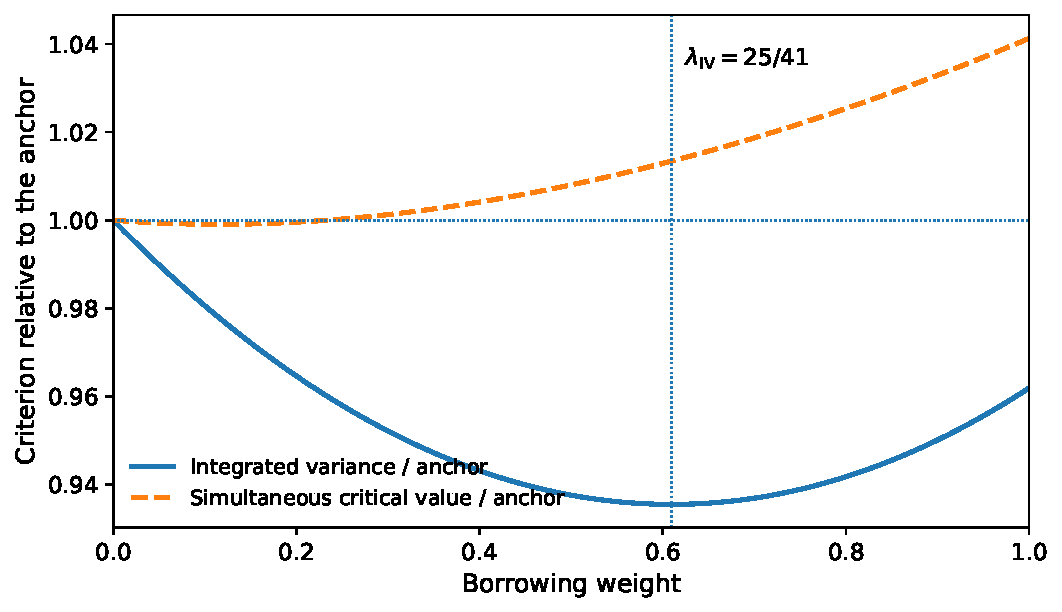
\includegraphics[width=.82\linewidth]{figure1_separation.pdf}
\caption{The exact two-threshold example separates the trace and simultaneous-band criteria. Both curves are relative to Anchor; at the trace optimum $25/41$, the simultaneous critical value exceeds the anchor value. These are Gaussian calculations, not Monte Carlo estimates.}\label{fig:separation}
\noindent Alt text: The trace improves while the simultaneous criterion worsens at the trace optimum.
\end{figure}


\subsection{An implementable paired calibration}
An independent gate sample $\sg$ estimates $\Omega$ and accounts for Anchor centring.
The centred gate residuals use $\wh F=\PP_{\sg}K_hU_0/\PP_{\sg}K_h$ and $\wh r_i=(U_{0,i}-\wh F,B_i)^\top$.
The gate estimates the covariance, centring derivative and Anchor influence contribution:
\begin{equation}\label{eq:moments}
 \wh\Omega=\frac p{v_h}\PP_{\sg}(K_h^2\wh r\wh r^\top),\quad
 \wh A=\frac p{v_h}\PP_{\sg}(K_h^2\wh r),\quad
 \wh\ell_i=\frac{K_{h,i}(U_{0,i}-\wh F)}{\PP_{\sg}K_h}.
\end{equation}
The covariance influence contribution explicitly incorporates the estimation of Anchor centring:
\begin{equation}\label{eq:covif}
 \wh C_i=\wh\Psi_i\wh\Psi_i^\top-\wh\Omega
       -E_0\wh\ell_i\wh A^\top-\wh A\wh\ell_i^\top E_0^\top,
       \qquad E_0=\binom{I_J}{0}.
\end{equation}

Let $\Lset$ be a finite weight grid containing zero, with normalised gain gradients defined for $\lambda>0$.
These gradients convert covariance influence contributions into scores for calibrating gain uncertainty:
\begin{equation}\label{eq:gradient}
 D_\lambda(\Omega)=\nabla_\Omega\{g_\Omega(\lambda)/\lambda\},\qquad
 \wh s_{i\lambda}=\inner{D_\lambda(\wh\Omega)}{\wh C_i}.
\end{equation}
Centre the scores across observations; independent standard normal multipliers approximate $\max\{0,\max_{\lambda>0}n_{\sg}^{-1}\sum_i\xi_i\wh s_{i\lambda}\}$.
Let $\wh t_\delta$ be an upper simulated quantile at probability $1-\delta$.
A nonnegative second-order cushion $b_N$ and fresh Gaussian intervals $[\underline c_\lambda,\overline c_\lambda]$ protect the plug-in critical-value comparison.
Paired selects the weight with the largest lower bound on simultaneous critical-value gain:
\begin{equation}\label{eq:rule}
 \wh L(0)=0,\quad
 \wh L(\lambda)=\underline c_0-\overline c_\lambda
                       -\lambda(\wh t_\delta+b_N),\quad
 \wh\lambda\in\argmax_{\lambda\in\Lset}\wh L(\lambda).
\end{equation}
Ties at zero select Anchor; comparisons share the same estimated joint covariance.
The numerical studies use $b_N=\wh c_0\log(1+k_G)/k_G$, where $k_G$ counts verified kernel-support observations, with $k_G$ replaced by one when zero.
Its asymptotic order under localisation is $\log N_G/N_G$, with local information index $N_G=n_Gph^d$.

Radial Gaussian integration evaluates the score gradient using the following probability representation.
For a Cholesky factor $L$ and a uniform direction $V$ on the unit sphere in $\R^J$,
\begin{equation}\label{eq:radial}
 \Pr\{\norm{N(0,\Sigma)}_\infty\leq t\}
 =\E_V F_{\chi_J}\{t/\norm{LV}_\infty\}.
\end{equation}
The Supplement derives the gradient and numerical conditions; fresh independent Gaussian draws provide the order-statistic intervals in \eqref{eq:rule}.
Their error probability enters the certificate separately from statistical calibration uncertainty.

\section{Certification and simultaneous inference}
\subsection{A covariance-set benchmark and paired sensitivity}
Conditional on training, let $\mathcal C_G$ be a nonempty compact set of positive semidefinite joint covariances with coverage at least $1-\delta$.
The paired lower bound compares critical values throughout this set and determines the ideal selector:
\begin{equation}\label{eq:ideal}
 L_G(\lambda)=\inf_{Q\in\mathcal C_G}\{c_Q(0)-c_Q(\lambda)\},\qquad
 \lambda_G\in\argmax_{\lambda\in\Lset}L_G(\lambda).
\end{equation}
Both critical values use the same $Q$, giving $L_G(0)=0$ exactly for the common comparison.
This benchmark separates the statistical certificate from the numerical approximation of its criterion.

\begin{theorem}[Paired certification]\label{th:ideal}
Let $\lambda^\star\in\argmax_{\lambda\in\Lset}g_\Omega(\lambda)$. Then
$\Pr\{g_\Omega(\lambda_G)<0\mid\sT\}\leq\delta$. On $\{\Omega\in\mathcal C_G\}$,
\begin{equation}\label{eq:genericregret}
 0\leq c_\Omega(\lambda_G)-c_\Omega(\lambda^\star)
 \leq\sup_{Q\in\mathcal C_G}|g_Q(\lambda^\star)-g_\Omega(\lambda^\star)|.
\end{equation}
Neither uniqueness nor curvature of the minimiser is required.
\end{theorem}
The inequalities $g_\Omega(\lambda_G)\geq L_G(\lambda_G)\geq L_G(\lambda^\star)$ and $L_G(\lambda_G)\geq0$ reduce the oracle comparison to paired covariance sensitivity.

\begin{theorem}[Anchor-adaptive sensitivity]\label{th:sensitivity}
Fix $J$, $\alpha$, $\kappa>0$ and $B<\infty$. Suppose $Q,Q'$ belong to
$\mathcal K_{\kappa,B}=\{Q\succeq0:\norm Q_\op\leq B,
H_\lambda QH_\lambda^\top\succeq\kappa I_J,\ 0\leq\lambda\leq1\}$.
There is a finite $C=C(J,\alpha,\kappa,B)$ such that
\begin{equation}\label{eq:pairedlip}
 |g_Q(\lambda)-g_{Q'}(\lambda)|\leq C\lambda\norm{Q-Q'}_\op.
\end{equation}
If $\mathcal C_G\subset\mathcal K_{\kappa,B}$ has radius $\varepsilon_G$ about a common centre, the right side of \eqref{eq:genericregret} is at most $2C\lambda^\star\varepsilon_G$.
\end{theorem}
The proof differentiates the Gaussian rectangle quantile twice with respect to covariance and uses the cancellation at $\lambda=0$.
The joint matrix may be singular, provided its output covariance is positive definite; this includes an exactly zero correction.
The constants depend on dimension and conditioning; growing grids require the explicit dimension-dependent conditions in the Supplement.

\subsection{Feasible calibration under scarce verification}
Write $N_G=n_Gph^d$ and $N_E=n_Eph^d$ for the local information indices governing the implemented procedure.
Within each triangular row, observations are independent copies and the three sample roles are disjoint.
Assume $\mu_h\asymp h^d$ with bounded kernels and candidate functions, together with verification bounds $0<c_e\leq e\leq C_e<\infty$.
Both information indices diverge, and output covariances remain in a compact positive definite set for fixed threshold and weight grids.
The normalised nonzero covariance-influence scores satisfy the Lindeberg and covariance-consistency conditions in Supplementary Section~S3.
These conditions apply to the fitted path and accommodate misspecification of either regression.

\begin{theorem}[Feasible paired calibration]\label{th:feasible}
Under these conditions, the covariance estimator in \eqref{eq:moments} has the influence expansion \eqref{eq:covif}, and
\begin{equation}\label{eq:slopelinear}
 \frac{g_{\wh\Omega}(\lambda)-g_\Omega(\lambda)}{\lambda}
   =\frac1{n_G}\sum_{i\in G}\inner{D_\lambda(\Omega)}{C_i}
     +O_P(N_G^{-1})
\end{equation}
uniformly over nonzero grid weights. Suppose $b_N\sqrt{N_G}\to0$ and $N_Gb_N\to\infty$, and the computed score gradients obey the consistency condition in Section~S3. If the numerical critical-value intervals fail jointly with probability at most $\eta_c$, and the simulated multiplier quantile fails as an upper quantile with probability at most $\eta_t$, then \eqref{eq:rule} satisfies
\begin{equation}\label{eq:asympsafety}
 \Pr\{g_\Omega(\wh\lambda)<0\mid\sT\}
       \leq\delta+\eta_c+\eta_t+o(1).
\end{equation}
There is an event $\mathcal A_N$ with conditional probability at least
$1-\delta-\eta_c-\eta_t-o(1)$ and a nonnegative $R_N=O_P(N_G^{-1/2})$ such that, on $\mathcal A_N$, every grid oracle $\lambda^\star$ satisfies
\begin{equation}\label{eq:feasible-regret}
 0\leq c_\Omega(\wh\lambda)-c_\Omega(\lambda^\star)
 \leq\lambda^\star(R_N+\wh t_\delta+b_N)+e_{\mc}(\lambda^\star).
\end{equation}
Here $\wh t_\delta=O_P(N_G^{-1/2})$, $e_{\mc}(\lambda)$ sums the anchor and candidate numerical interval widths, and $e_{\mc}(0)=0$. The bound retains the certificate's failure probability; at an anchor oracle its zero regret is asserted on $\mathcal A_N$.
\end{theorem}
Theorem~\ref{th:ideal} gives finite-sample covariance-set certification, whereas Theorem~\ref{th:feasible} gives the implemented asymptotic multiplier guarantee.
Exact finite-sample protection covers Monte Carlo quantile errors; Section~S2 supplies an observable Bernstein covariance ball for the benchmark.
For $D=s_N\widetilde D$ with $s_N\to0$, the score statement applies after normalisation by the nonzero path scale under the corresponding Lindeberg condition.
The case $D=0$ returns Anchor exactly under the implemented rule.

\subsection{Coverage, whole distributions and rotating roles}
\begin{theorem}[Independent evaluation]\label{th:coverage}
Let $\mathcal L\subseteq[0,1]$ be a fixed finite set or the compact interval. Assume the evaluation score process admits a Gaussian approximation uniformly over $\lambda\in\mathcal L$, its covariance estimate is uniformly consistent, and its Gaussian maximum is uniformly continuous at the target quantiles. For any $\mathcal L$-valued weight measurable with respect to the training and selection samples, the independently calibrated grid band has coverage at least $1-\alpha-\eta_E-o(1)$, where $\eta_E$ bounds its Monte Carlo quantile error. No convergence to a unique deterministic weight is needed.
\end{theorem}
Conditional on training and gate data, the chosen weight is fixed in \eqref{eq:identity}.
Uniform Gaussian approximation and covariance consistency then establish the evaluation result.
With a uniformly bounded local score envelope, Gaussian rectangle bounds apply when $\log^7(n_EJ)/N_E\to0$ \citep{cck2016clt}.
Continuous-index results use the local increment and entropy conditions in Section~S4.

If grid limits $(l_j,u_j)$ cover $F_h(y_j)$, define their whole-distribution envelopes by
\begin{equation}\label{eq:envelope}
 l(y)=\max\{0,\max_{y_j\leq y}l_j\},\qquad
 u(y)=\min\{1,\min_{y_j\geq y}u_j\}
\end{equation}
These envelopes cover the entire distribution, taking empty maxima and minima as zero and one.
Inverting these envelopes gives simultaneous quantile bounds even at atoms, with the resulting width depending on grid resolution.
A second-order localisation bias is negligible for the point target when $\sqrt{N_E}h^2\to0$; smooth positive density additionally gives the quantile-process derivative.

Calibrate each of three roles at error $\alpha/3$ and intersect their whole-distribution bands.
A union bound gives overall error at most $\alpha+o(1)$ with arbitrary dependence between those bands.
Section~S5 also gives valid convex combinations of endpoints, which can be wider.

\subsection{How much reference information certifies a gain?}
Consider equally likely $S\in\{-1,1\}$ and the binary indicator $Z=\ind(Y=0)$, with
$\Pr_\theta(Z=1\mid S)=1/2+\theta S$. Set $q=1/2$, $D=dS$, $0<d<1/4$, and verify independently with probability $p$.
The scaled augmentation variance along this path has the following form:
\begin{equation}\label{eq:binary}
 p\Var_\theta(U_\lambda)=\tfrac14+(1-p)(d^2\lambda^2-2d\theta\lambda).
\end{equation}
For $0<\theta<d$, $\lambda^\star=\theta/d$ and the optimal critical-value gain is
$z_{1-\alpha/2}(1-p)\theta^2+O(\theta^4)$.

\begin{theorem}[Local certification boundary]\label{th:boundary}
If a positive-gain certificate is issued on an event $A$ with $\Pr_0(A)\leq\delta$, then
$\Pr_\theta(A)\leq\delta+\sqrt{2n_Gp}|\theta|$.
Localising the association to a box-kernel support of probability $r_h$ replaces $n_Gp$ by $n_Gpr_h$. Conversely, conditional on $k$ local verified observations,
\begin{equation}\label{eq:binarycert}
 \theta_L=\frac1{2k}\sum_{i=1}^k S_i(2Z_i-1)
        -\sqrt{\frac{\log(1/\delta)}{2k}},\qquad
 \wh\lambda=\min\{1,(\theta_L)_+/d\}
\end{equation}
has harmful-selection probability at most $\delta$, and selects a positive weight with probability at least $1-\beta$ if
$\theta\geq\sqrt{\log(1/\delta)/(2k)}+\sqrt{\log(1/\beta)/(2k)}$.
\end{theorem}
The proof bounds observed-data divergence by $4n_Gp\theta^2$ and uses a one-sided Hoeffding bound for the converse.
In this submodel, the signal boundary is $N_G^{-1/2}$ and the oracle-gain boundary is $N_G^{-1}$.
Retaining this resolution requires smaller numerical error and a weight mesh that resolves the local optimum.

\section{Simulation study}
\label{sec:simulation}
\subsection{Design, comparators and performance measures}
The experiments separate three questions about borrowing: improvement in distribution estimation, reduction in simultaneous band width and support for a positive-gain certificate.
Methods share observations, verification indicators and role assignments within each replication.
Twelve cells use 500 replications each; Supplementary Table~S1 reports the complete results.
Table~\ref{tab:simulation} compares all six methods at a common sample size and reference fraction.

We independently generate $X\sim U[-1,1]$, $\varepsilon,\eta\sim N(0,1)$ to form the reference outcome and surrogate:
\[
 Y=\mu(X)+\sigma(X)\varepsilon,\quad
 \mu(x)=1.2x+0.6x^2,\quad \sigma(x)=0.8+0.25x^2,\quad
 S=\ell(X)Y+\tau\eta.
\]
Alignment uses $\ell(x)=1$ and $\tau=0.4$; the weak-surrogate design changes $\tau$ to 1.6.
The local-reversal design sets $\ell(x)=-1$ for $|x|\leq0.4$ and $\ell(x)=1$ elsewhere.
The no-signal design takes $\ell(x)=0$; the zero-path design sets the surrogate candidate equal to Anchor.

The target is $F_h(\cdot\mid0)$ with an Epanechnikov kernel, $h=0.35$, and seven thresholds $0.8\Phi^{-1}(u_j)$.
The $u_j$ are equally spaced from 0.1 to 0.9, with weight grid $\{0,0.1,\ldots,1\}$.
Sample sizes are 6,000 and 12,000, with reference fractions 0.05, 0.10 and 0.20.
Bounded selective verification favours larger standardised surrogate readings; Section~S9 gives its probability for comparison with random verification.
Three equal roles fit Gaussian location--scale regressions, select borrowing and evaluate the distribution.
Anchor uses mean features $(1,X,X^2)$; the surrogate mean additionally uses $S$.

Anchor and Full fix $\lambda=0$ and 1, respectively, throughout each replication.
Trace minimises the estimated covariance trace; Plug-in directly minimises the estimated simultaneous critical value.
Projection estimates a matrix control variate from the same gate covariance, using ridge $0.05\tr(\wh\Omega_{11})/J$.
Its matrix mixes and reverses threshold corrections, extending the scalar candidate class.
Paired uses \eqref{eq:rule}, with statistical selection error 0.049 and two numerical selection errors of 0.0005 each.
Evaluation allocates 0.049 to Gaussian coverage and 0.001 to numerical calibration.
Radial gradients use 8,192 directions, gate calibration uses 3,999 multiplier draws, and critical-value protection uses 32,768 independent Gaussian draws.

We report simultaneous coverage, within-replication band-width ratios to Anchor, selected weights and grid-integrated squared error (ISE),
\[
 \operatorname{ISE}_{J}=J^{-1}\sum_{j=1}^J
       \{\wh F_h(y_j)-F_h(y_j)\}^2,
\]
using the raw estimator on the inferential grid in every comparison.
Harmful selection means $c_\Omega(\wh\lambda)>c_\Omega(0)+10^{-4}$ for the population covariance of the fitted path.
Deterministic quadrature evaluates the covariance and its Gaussian criteria for this assessment.
Continuous summaries use independent-replication Monte Carlo standard errors (MCSE); coverage and harm frequencies receive binomial intervals.

\subsection{Gains, reversal and the cost of certification}
Across twelve cells, Paired coverage ranges from \SimCovMin{} to \SimCovMax{}, with aligned mean width ratios \SimAlignedWidthMin{}--\SimAlignedWidthMax{}.
At $n=6,000$ and $p=0.10$ under random verification, grid ISE falls from $3.074\times10^{-3}$ for Anchor to $1.567\times10^{-3}$ for Paired, whose width ratio is 0.747.
Full, Trace and Plug-in yield width ratios near 0.722 and grid ISE near $1.42\times10^{-3}$.
Paired's mean weight rises from 0.507 to 0.807 as $p$ increases from 0.05 to 0.20; adoption rises from 0.862 to 1.000.
Doubling the sample size at $p=0.10$ raises mean weight from 0.718 to 0.822 and reduces the width ratio from 0.747 to 0.731.
Under selective verification at $p=0.05$, adoption is 0.752 and mean weight is 0.421.

Full has width ratio 0.954 and grid ISE $2.526\times10^{-3}$ against $2.899\times10^{-3}$ for Anchor.
Paired chooses zero in all 500 replications under the stated budgets.

Full increases mean width by 11.4\% and grid ISE from $3.080\times10^{-3}$ to $3.909\times10^{-3}$, with harmful-selection frequency 0.994.
Paired returns Anchor; Trace and Plug-in select positive borrowing in only 0.6\% of replications.
Projection has width ratio 0.805 and grid ISE $1.901\times10^{-3}$ in this setting.
Under no signal, Trace and Plug-in have harmful-selection frequencies 0.310 and 0.312 and mean Gaussian gains $-0.000217$ and $-0.000232$, respectively.
Their width ratios are near 1.000, and Paired records no harmful selections.
Projection has width ratio 1.013 and mean gain $-0.007431$; every method reduces to Anchor in the exact zero-path cell.

\begin{figure}[htbp]\centering
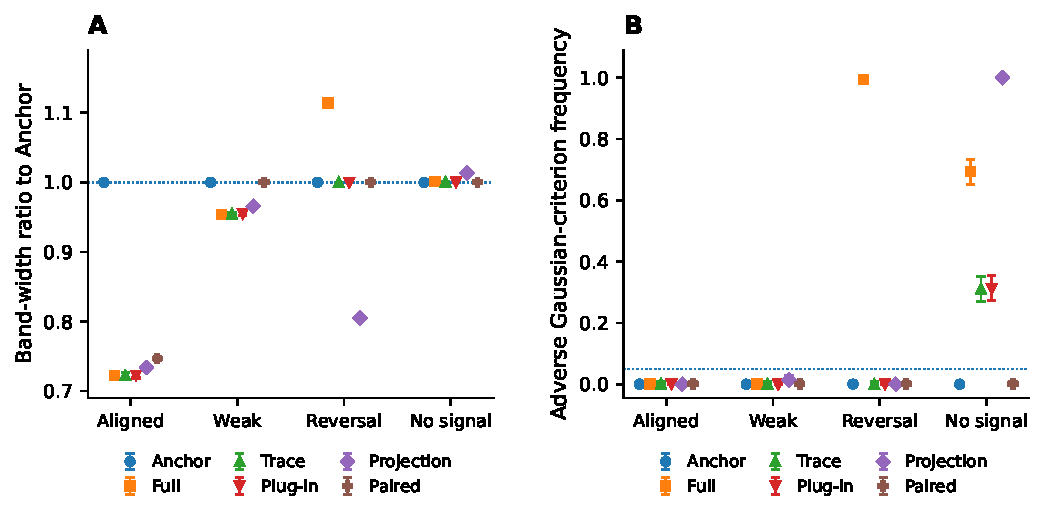
\includegraphics[width=\linewidth]{v2/figure2_simulation_comparison.pdf}
\caption{Six-method comparisons with $n=6,000$ and $p=0.10$ under random verification. (A) Mean within-replication band-width ratios; bars are $\pm1.96$ Monte Carlo standard errors. (B) Assessed harmful-selection frequencies, using critical-value tolerance $10^{-4}$; bars are exact binomial 95\% intervals. Each mechanism has 500 replications. The dotted reference in (B) is 0.05.}\label{fig:simulation_comparison}
\noindent Alt text: Projection benefits from reversal; Paired retains Anchor under weak and absent signals. Near-null harm frequencies can be high despite small width changes.
\end{figure}


\subsection{Pairing, dense thresholds and robustness}
Six additional cells with 500 replications each compare Paired with Unpaired under a matched design.
Unpaired separately bounds the Anchor critical value and the candidate-critical-value maximum; Section~S3.5 establishes error control.
Both selectors share fitted candidates, samples, weight meshes, numerical critical-value intervals and the total $0.05$ selection-error budget.
Unpaired adds two absolute-error bounds; Paired calibrates their difference using the gate scores.
Under alignment at $p=0.05,0.10,0.20$, Paired's width ratios are 0.802, 0.747 and 0.769 against 1.000, 1.000 and 0.993 for Unpaired.
Adoption probabilities are 0.858, 0.998, 1.000 for Paired and 0.000, 0.000, 0.032 for Unpaired.
Both rules return Anchor under reversal and the no-signal correction.
Paired coverage is 0.928--0.958, with low Anchor coverage in the weakest cell; Section~S10 gives exact binomial intervals and all six-method comparisons.

The dense-grid experiment uses 21, 51 and 101 nested thresholds spanning probabilities $0.02$--$0.98$ under alignment and selective local reversal.
Each mechanism uses 200 datasets shared across resolutions and covariance enlargement $10^{-8}I_J$.
Paired coverage is 0.935 to 0.965, with aligned width ratios 0.765, 0.782 and 0.798; it retains Anchor under reversal.
The common 1,001-point grid evaluates monotone envelopes beyond the seven-coordinate primary experiment.

Seven further cells with 300 replications each examine standardised $t_3$, skewed and mixture errors, a ten-category outcome, two-dimensional localisation, neighbour-distribution candidates and fitted logistic verification probabilities.
The six known-design cells give Paired coverage 0.950--0.970 and width ratios 0.686--0.841.
The learned-probability sensitivity gives coverage 0.963 and width ratio 0.768 under the nuisance-drift conditions in Section~S8.
Each generating distribution supplies the complete conditional CDF, including ordinal cutpoints.

\begin{figure}[htbp]\centering
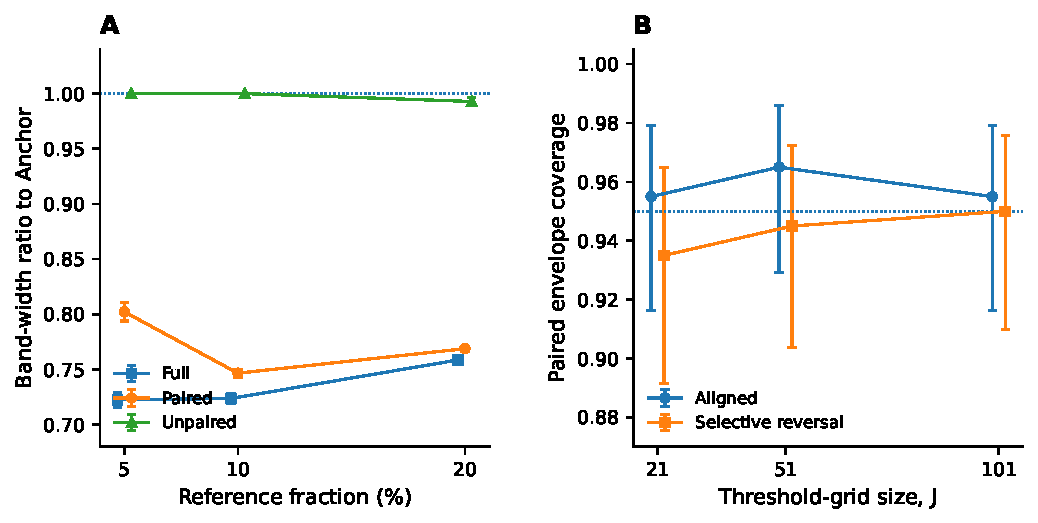
\includegraphics[width=\linewidth]{v3/validation.pdf}
\caption{Pairing and dense-threshold validation. (A) Mean width ratios in the matched ablation, with $\pm1.96$ Monte Carlo standard errors of within-replication ratios, 500 replications per budget. Both certified rules use the same total error budget. (B) Paired monotone-envelope coverage on a common 1,001-point evaluation grid; bars are exact cellwise binomial 95\% intervals. The 200 datasets per mechanism are shared across threshold resolutions.}\label{fig:validation}
\noindent Alt text: Paired retains substantially more width improvement than the unpaired bound. Dense-grid envelope coverage is close to nominal, with visible Monte Carlo uncertainty.
\end{figure}


\subsection{Exact operating characteristics, rotation and numerical checks}
Theorem~\ref{th:boundary} permits exact binary calculations independently of covariance quadrature and its numerical precision.
With $p=0.1$, correction amplitude $d=0.2$ and certification error 0.05, we evaluate eight verified counts from 25 to 3,200.
Eight associations run from $-0.04$ to 0.15; the 192 method--configuration entries are binomial probability sums.
Figure~\ref{fig:binary_certification} shows error control and adoption across the evaluated configurations.
At zero association, Plug-in harmful-selection probability is 0.444 for $k=50$ and 0.493 for $k=3,200$.
The exact binomial rule gives 0.032 and 0.047, and Hoeffding gives approximately 0.008 and 0.007.
The largest error among both lower-bound rules over the grid is 0.0494.
For $\theta=0.04$, exact-binomial adoption rises from 0.100 at $k=50$ to 0.727 at $k=800$ and 0.998 at $k=3,200$.
Corresponding Hoeffding adoption probabilities are 0.031, 0.430 and 0.981 across those counts.

\begin{figure}[htbp]\centering
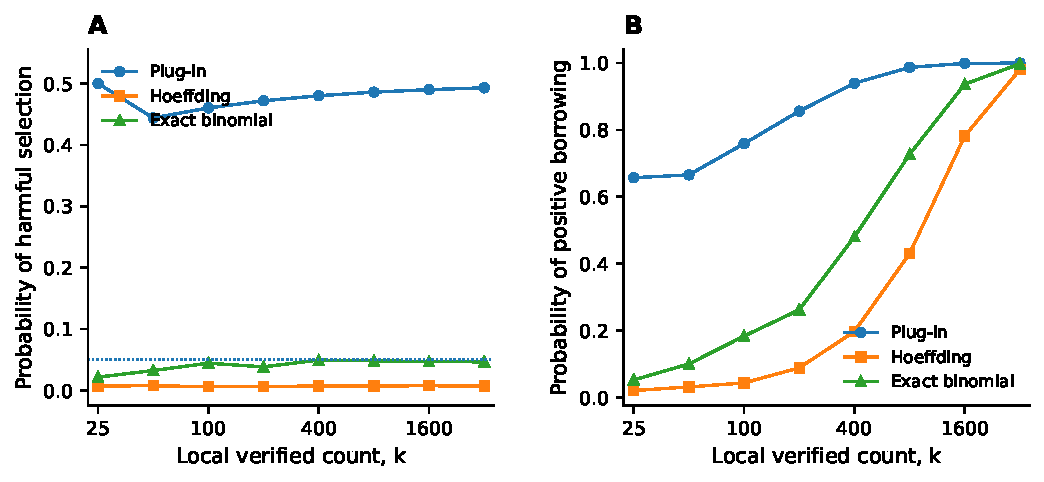
\includegraphics[width=\linewidth]{v2/figure3_binary_certification.pdf}
\caption{Exact binomial operating characteristics of the local submodel, with $p=0.1$, $d=0.2$ and certification error 0.05. (A) Harmful selection at $\theta=0$. (B) Positive borrowing at $\theta=0.04$. All values are exact binomial sums; the two lower-bound rules have distinct power despite controlling error.}\label{fig:binary_certification}
\noindent Alt text: Plug-in harm approaches one half under the null; certified adoption increases with the verified count under a weak positive association.
\end{figure}


A separate 400-replication experiment uses 200 aligned and 200 reversed datasets with the dependence-valid intersection of three role-specific bands.
Under alignment, Anchor and Paired coverage is 0.960 and 0.970, with mean widths 0.264 and 0.202.
Under reversal, both methods have coverage 0.975 and mean width 0.263.
Convex endpoint aggregation is wider and covers in every replication; Section~S5 defines this separate experiment's construction.

All 6,000 primary replications finished successfully, and none required an information fallback.
Across 60 checks, increasing radial directions from 8,192 to 32,768 preserved every Paired selection, with largest critical-value change $3.935\times10^{-4}$.
The additional 6,300 design--grid replications use 5,500 distinct datasets because dense resolutions share samples.
Refinement in 30 dense-grid cases changes the selected mesh point in 5 cases, with largest evaluation-width change 3.26\% and estimated CDF change 0.0063.
Section~S10 retains all numerical comparisons, including every observed selection disagreement.

\section{Humidity-specific air-monitor calibration}
\label{sec:application}
\subsection{Scientific question and historical calibration}
Can a mean-calibrated low-cost particle sensor recover the reference instrument's exceedance frequencies, and which discrepancies can a limited reference sample establish?
The United States Environmental Protection Agency (EPA) study collocated six particulate-matter sensor types with reference instruments at seven United States sites \citep{Barkjohn2025}.
Processed PurpleAir data provide 2,814 complete site-days from 22 July 2019 to 1 January 2021, covering 530 dates and 76 calendar weeks.
Date recovery preserves the original observation identifiers and confirms unique site--date combinations.
The target is the processed collocation series, retaining the source quality-control exclusions.

All 985 site-days in 2019 fit the historical calibration, which we freeze before subsequent distributional verification:
\begin{equation}\label{eq:epacal}
 \widetilde S=3.098+0.486S-1.127(X-50)/20,
\end{equation}
where $S$ is uncorrected sensor concentration in micrograms per cubic metre and $X$ is relative humidity in percent.
Full-precision coefficients are stored in code; the remaining 1,829 site-days form the 2020--2021 audit frame.
The same historical sample fits Anchor and surrogate distribution regressions.
Their predictions and the calibration equation are frozen before reference sampling in the audit frame.
The initial 985 reference measurements are additional to subsequent audit budgets.

Outcome regressions model $\log(1+Y)$, where $Y$ denotes reference concentration before transformation.
Anchor uses humidity terms; the surrogate candidate adds sensor concentration and its interactions, with a fitted scale regression.
Concentration thresholds are transformed inside these regressions, while scientific effects and intervals are reported on the original concentration scale.
The archived whole-series leave-one-site-out diagnostic uses a different training design and is kept separate from this analysis.

\subsection{The distributional target and complete-frame discrepancies}
Kernel weights $K_i(r)=K\{(X_i-r)/10\}$ define the local contrast between reference and corrected-sensor distributions:
\begin{equation}\label{eq:epatarget}
 \Delta_H(t;r)=\frac{\sum_{i\in H}K_i(r)
       \{\ind(Y_i\leq t)-\ind(\widetilde S_i\leq t)\}}
       {\sum_{i\in H}K_i(r)}.
\end{equation}
The contrast measures corrected-sensor minus reference exceedance frequency; positive values indicate overstatement in each humidity neighbourhood.
The humidity targets $r=30\%,50\%,70\%$ use the seven inferential concentration thresholds $5,10,15,20,25,30,40$.
The thresholds specify concentration levels used to assess distributional calibration.
Nonzero kernel supports contain 379, 783 and 482 site-days before reference subsampling.
The kernel effective sample sizes $(\sum K_i)^2/\sum K_i^2$ are 315.889, 658.420 and 403.199, respectively.

Table~\ref{tab:epa_science} reports complete-frame calibration at $30\%$ humidity: mean corrected-minus-reference concentration difference $-0.191$ and 0.90-quantile difference $-1.612$.
At concentration 15, corrected and reference exceedance frequencies are $6.068\%$ and $9.307\%$, a difference of $-3.239$ percentage points.
At $70\%$ humidity, mean difference is $-0.227$, 0.90-quantile difference is $+0.471$, and exceedance discrepancy at 15 is $+1.157$ percentage points.

In Figure~\ref{fig:epa}, the discrepancy at $30\%$ humidity changes from positive to negative, reaching 18.602 percentage points at concentration 5.
Colorado receives 43.462\% of kernel weight at $30\%$ humidity and 0.793\% at $70\%$.
The target retains the recorded station--day mixture within each humidity neighbourhood.

\begin{figure}[htbp]\centering
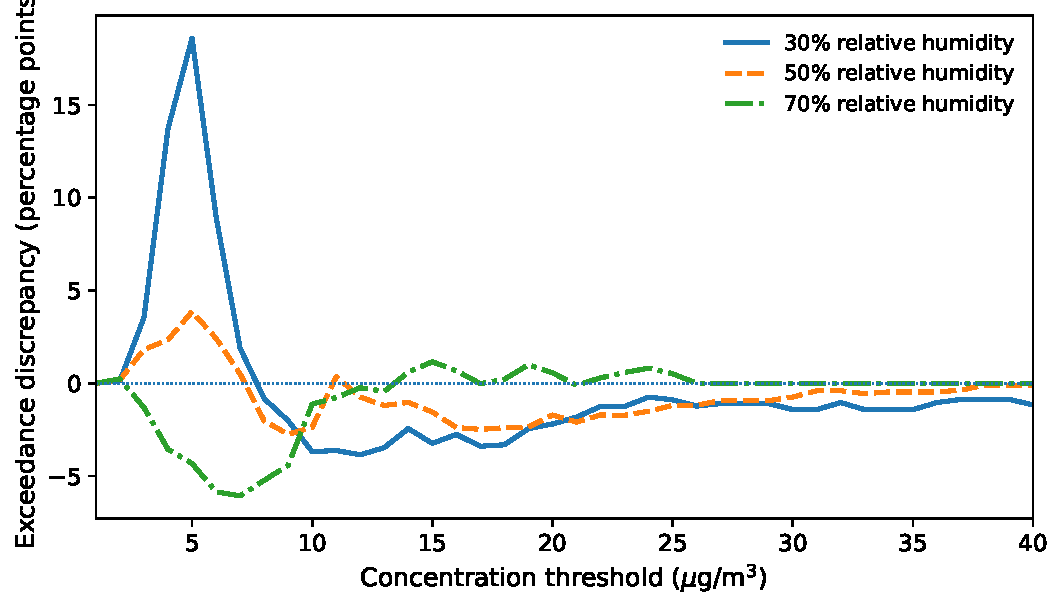
\includegraphics[width=.86\linewidth]{figure2_epa_discrepancy.pdf}
\caption{Complete-frame exceedance discrepancies after historical mean calibration. Positive values indicate overstatement by the corrected sensor. The curves use 40 integer concentration thresholds; inference uses the separately declared seven-threshold grid. These full-reference descriptions have no confidence limits.}\label{fig:epa}
\noindent Alt text: The discrepancy changes sign across concentration thresholds and differs among humidity neighbourhoods.
\end{figure}


\subsection{Designed verification and finite-frame intervals}
We independently randomise gate and evaluation masks conditional on the audit frame, giving design-based uncertainty for that frame.
For a unit-specific union probability $p_i$, the two role probabilities are
\begin{equation}\label{eq:twomasks}
 \pi_{G,i}=p_i/2,\qquad
 \pi_{E,i}=\frac{p_i-\pi_{G,i}}{1-\pi_{G,i}},
\end{equation}
so $\Pr(R_{G,i}\vee R_{E,i}=1)=p_i$ under independent gate and evaluation sampling.
Random auditing uses $p_i=p$; selective auditing uses a bounded sensor-level score normalised to mean $p$, with budgets $p=0.05,0.10,0.20$.
Common uniforms nest each role's samples across budgets, and all five methods share the same masks.
A unit selected by both roles is measured once towards the unique reference budget.
The masks remain independent conditional on the audit frame, including when their realised selections overlap.

Evaluation replaces reference indicators in \eqref{eq:epatarget} by $U_{\lambda,t}$ using $R_E/\pi_E$.
With $w_i=K_i/\overline K$, $d_i=m_i-q_i$ and $r_i=(q_i-Z_i,d_i)^\top$, the joint matrix generates design covariance scaled by $np$:
\begin{equation}\label{eq:epacov}
 \Omega_H=\frac pn\sum_{i\in H}w_i^2(\pi_{E,i}^{-1}-1)r_ir_i^\top.
\end{equation}
The gate weights summands by $R_{G,i}/\pi_{G,i}$ and uses Bernoulli-design covariance-influence scores for paired calibration; Section~S6 derives this calculation.
Corrected-sensor indicators are known throughout the audit frame and cancel from its randomisation error.

Two hundred masks in each of six design--budget cells give 1,200 reference-sampling repetitions.
Error budgets cover all 21 threshold--humidity combinations across the three humidity targets.
The common Gaussian enlargement $10^{-8}I$ handles tail-grid singularities and preserves point estimates.
Complete audit outcomes enter performance evaluation only; neighbourhoods with fewer than three evaluation references receive full feasible distribution bands that remain included in coverage.

Supplementary Figure~S1 shows the first retained random-audit mask at 20\%, with 369 unique reference measurements.
The gate/evaluation counts are 31/39, 72/104 and 48/66, and Paired weights are 0, 0.8 and 0.
At $50\%$ humidity, Paired width is 15.881 percentage points against 27.632 for Anchor and 14.831 for Full.
Paired retains Anchor at $30\%$ and $70\%$; the $70\%$ interval at concentration 10 misses the complete-frame value.

Table~\ref{tab:epa_budget} compares five methods, including the two unprotected adaptive selectors.
Paired joint coverage is 0.935--0.970 across the six evaluated design--budget cells.
The 0.935 result has Monte Carlo standard error 0.017, with exact binomial intervals retained for the comparisons.
Under random auditing, Full has humidity-averaged width ratios 0.679, 0.667 and 0.660, against 0.985, 0.942 and 0.828 for Paired.

At the 5\% random budget, the $30\%$ humidity gate averages 9.93 references and Paired adoption is 1.5\%.
At the 20\% budget, mean gate support rises to 38.46 and adoption to 40.5\%.
At $50\%$ humidity, the counts are 19.67 and 77.37, with adoption rates 10.5\% and 81.5\%.
Mean unique audit budgets are about 91, 183 and 365 measurements, in addition to the historical 985.

\subsection{Reference budgets and upper-tail precision}
A sign is resolved only when its simultaneous interval excludes zero in the correct direction.
At $30\%$ humidity and concentration 5, Paired resolution is 1.0\%, 9.5\% and 68.0\% under 5\%, 10\% and 20\% random audit budgets.
Corresponding frequencies are 1.0\%, 8.0\% and 52.0\% for Anchor and 32.0\%, 55.0\% and 89.0\% for Full.
At concentration 15 and the 20\% budget, Paired resolution is 0\%, 0.5\% and 0\% across humidity targets.
These complete-frame differences are smaller than the discrepancy at concentration 5.
All 126,000 method--mask--threshold records, including false-sign events, remain available for the evaluated grid.

\begin{figure}[htbp]\centering
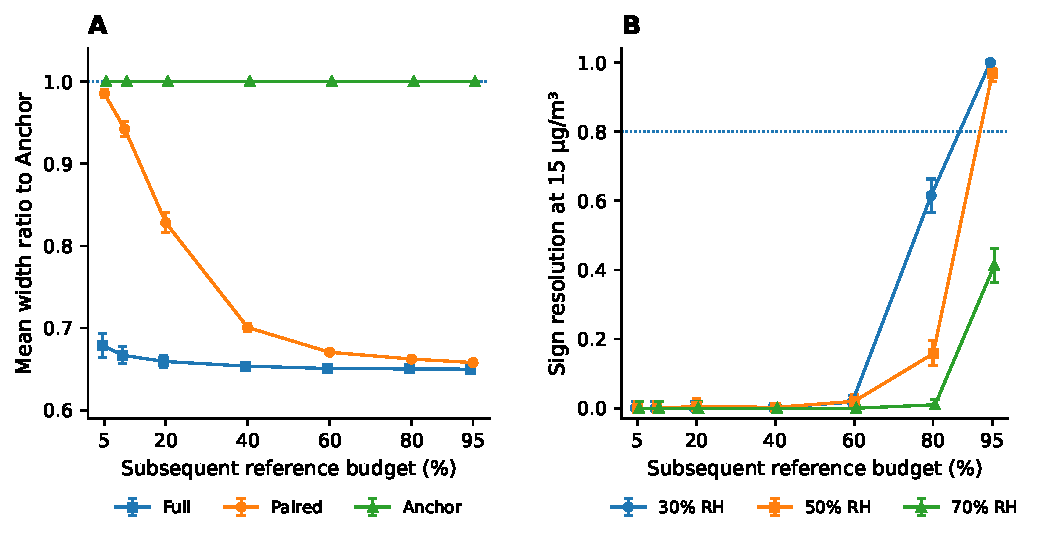
\includegraphics[width=\linewidth]{v3/epa_budget_full.pdf}
\caption{Reference-budget and upper-tail precision under random auditing. (A) Width ratios averaged across humidity within each mask, with $\pm1.96$ Monte Carlo standard errors. (B) Paired's correct sign resolution at concentration 15, with exact binomial 95\% intervals; the dotted line is 0.80. Budgets 5--20\% use the original 200 masks and budgets 40--95\% use 400 masks. Draw families are nested across budgets; historical training costs are additional.}\label{fig:epa_budget}
\noindent Alt text: Increasing reference budgets allows smaller upper-tail differences to be resolved, but the 70-percent humidity discrepancy remains unresolved in many masks even at a 95-percent budget.
\end{figure}


A fixed follow-up evaluates 40\%, 60\%, 80\% and 95\% budgets through 400 nested random-audit masks per budget.
The follow-up retains all low-budget results and keeps historical regressions, thresholds, humidity targets and the selector unchanged.
The 1,600 budget--mask combinations use four budgets sharing each of 400 independent uniform-draw families.

At concentration 15, Paired resolution probabilities at $p=0.80$ are 0.615, 0.158 and 0.010 across humidity targets.
At $p=0.95$, they are 1.000, 0.968 and 0.412, the last with exact 95\% Monte Carlo interval [0.364, 0.462].
Among evaluated subcensus budgets, 95\% first exceeds 80\% observed resolution at 30\% and 50\% humidity.
No evaluated subcensus budget reaches that resolution at 70\% humidity.
A complete reference census determines the finite-frame contrast exactly as a separate endpoint.
Joint coverage over all 21 combinations is 0.948--0.975; Figure~\ref{fig:epa_budget} displays the complete budget trajectory.
The 95\% budget uses about 1,737 distinct audit references in addition to the historical 985.
The precision assessment retains all thresholds, incorrect-sign events and Monte Carlo intervals.

\section{Discussion}
Pairing candidate and Anchor critical values ties gain uncertainty to the amount borrowed.
This cancellation makes the feasible multiplier calibration responsive to local reference information.

Under a common error budget, the matched ablation shows that a gain can be estimable as a difference while separate bounds remain too wide.
Dense-grid and non-Gaussian experiments show that this mechanism extends beyond a short threshold vector.

The candidate class determines the available efficiency gains and their certification cost.
Projection can exploit a reversed relationship outside the nonnegative scalar path, while Full can be more efficient under strong alignment.
Paired controls whether the fitted correction is used along the proposed path.
Insufficient gate information can leave a useful weak-surrogate correction uncertified under the stated confidence and numerical budgets.

Historical mean calibration and subsequent distributional verification answer different questions in the air-monitoring study.
A modest audit establishes a large lower-concentration discrepancy; a one-percentage-point upper-tail difference can require nearly complete verification under the same simultaneous family.
Designed reference sampling attributes this precision requirement to the audit frame and its recorded station--day mixture.

\section*{Data availability}
The EPA analysis table, source-verified date mapping and original computational archive are available in the public repository \url{https://github.com/Stork343/surrogate-assisted-local-conditional-distribution-inference}, source commit \texttt{70c47c512ab485edf502f16914f9ff481cc6be88}. The V3 reproduction package dated 29 September 2026 accompanying this manuscript contains the revised code, all generated results, input checksums and commands for rebuilding its tables and figures. The processed audit population and the historical calibration sample are identified separately.

\section*{Acknowledgements and funding}
This work was partially supported by the Beijing Natural Science Foundation (1242005), the Fundamental Research Funds for the Central Universities and the Research Funds of Renmin University of China (25XNN015), and the Ministry of Education Humanities and Social Sciences Research General Project (25YJA910005).

ChatGPT assisted the methodological revision, mathematical derivations, software development, numerical checks and drafting. Earlier computational development also used OpenAI Codex. These tools are not authors; responsibility for the submitted research, analysis and text rests with the authors.

\section*{Conflict of interest}
The authors declare no conflicts of interest.

\section*{Supplementary material}
The Supplement provides proofs, primitive and growing-grid conditions, numerical calibration details, rotating-role inference, the design-based audit extension and complete numerical results. The reproduction package provides executable code and the input and output data.

\bibliographystyle{plainnat}
\bibliography{references}
\clearpage\begin{table}[p]\centering\setstretch{1.0}
\caption{All six methods at a common sample size and reference fraction.}\label{tab:simulation}
\setlength{\tabcolsep}{3pt}
\begin{tabular}{llrrrr}\toprule
Mechanism & Method & Coverage & Grid ISE & $\Delta$ ISE (MCSE) & Gain \\\midrule
Aligned & Anchor & 0.956 & 3.074 & 0.000 (0.000) & 0.000 \\
 & Full & 0.960 & 1.419 & -1.656 (0.123) & 180.739 \\
 & Trace & 0.962 & 1.420 & -1.654 (0.121) & 180.373 \\
 & Plug-in & 0.962 & 1.427 & -1.647 (0.120) & 179.937 \\
 & Projection & 0.958 & 1.482 & -1.592 (0.121) & 172.550 \\
 & Paired & 0.956 & 1.567 & -1.508 (0.103) & 162.655 \\
\addlinespace[3pt]
Weak & Anchor & 0.960 & 2.899 & 0.000 (0.000) & 0.000 \\
 & Full & 0.966 & 2.526 & -0.373 (0.072) & 31.131 \\
 & Trace & 0.964 & 2.575 & -0.324 (0.058) & 29.995 \\
 & Plug-in & 0.962 & 2.580 & -0.318 (0.056) & 29.746 \\
 & Projection & 0.960 & 2.677 & -0.222 (0.063) & 23.600 \\
 & Paired & 0.960 & 2.899 & 0.000 (0.000) & 0.000 \\
\addlinespace[3pt]
Reversal & Anchor & 0.954 & 3.080 & 0.000 (0.000) & 0.000 \\
 & Full & 0.958 & 3.909 & 0.829 (0.063) & -72.220 \\
 & Trace & 0.954 & 3.080 & 0.000 (0.000) & 0.081 \\
 & Plug-in & 0.954 & 3.080 & 0.000 (0.000) & 0.081 \\
 & Projection & 0.966 & 1.901 & -1.178 (0.106) & 125.115 \\
 & Paired & 0.954 & 3.080 & 0.000 (0.000) & 0.000 \\
\addlinespace[3pt]
No signal & Anchor & 0.968 & 3.000 & 0.000 (0.000) & 0.000 \\
 & Full & 0.968 & 3.006 & 0.007 (0.009) & -0.683 \\
 & Trace & 0.966 & 3.003 & 0.003 (0.004) & -0.217 \\
 & Plug-in & 0.966 & 3.005 & 0.005 (0.005) & -0.232 \\
 & Projection & 0.958 & 3.105 & 0.105 (0.030) & -7.431 \\
 & Paired & 0.968 & 3.000 & 0.000 (0.000) & 0.000 \\
\bottomrule\end{tabular}
\par\raggedright\noindent Each row uses 500 replications with $n=6,000$ and random verification at $p=0.10$. Grid ISE, its mean paired difference from Anchor ($\Delta$ ISE) and mean Gaussian critical-value gain are multiplied by $10^3$. MCSE is the paired-difference Monte Carlo standard error. Negative $\Delta$ ISE and positive gain indicate improvement; Figure~\ref{fig:simulation_comparison} reports widths and harmful-selection frequencies. Supplementary Table~S1 contains all twelve cells and Monte Carlo uncertainties.
\end{table}
\begin{table}[p]\centering\setstretch{1.0}
\caption{Complete-frame calibration after historical training.}\label{tab:epa_science}
\setlength{\tabcolsep}{4pt}
\begin{tabular}{rrrrrr}\toprule
RH (\%) & Local rows & Mean diff. & $Q_{.90}$ diff. & Ref. $>15$ & Sensor $>15$ \\\midrule
30 & 379 & -0.191 & -1.612 & 9.307 & 6.068 \\
50 & 783 & -0.380 & -0.493 & 7.993 & 6.439 \\
70 & 482 & -0.227 & 0.471 & 7.038 & 8.194 \\
\bottomrule\end{tabular}
\par\raggedright\noindent Differences are corrected sensor minus reference in $\mu\mathrm{g}/\mathrm{m}^3$; exceedance frequencies are percentages. The frame has 1,829 site-days and the historical training sample 985. These are complete-frame descriptions.
\end{table}
\begin{table}[p]\centering\setstretch{1.0}
\caption{All five methods in the EPA reference-sampling experiment.}\label{tab:epa_budget}
\setlength{\tabcolsep}{4pt}
\begin{tabular}{lrrrrrr}\toprule
 & & \multicolumn{5}{c}{Method}\\
Design & $p$ (\%) & Anchor & Full & Trace & Plug-in & Paired \\\midrule
\multicolumn{7}{l}{(a) Joint coverage over all 21 threshold--humidity combinations}\\
Random & 5 & 0.960 & 0.995 & 0.995 & 0.995 & 0.960 \\
Random & 10 & 0.955 & 0.970 & 0.965 & 0.970 & 0.960 \\
Random & 20 & 0.970 & 0.975 & 0.975 & 0.970 & 0.970 \\
Selective & 5 & 0.955 & 0.990 & 0.975 & 0.980 & 0.955 \\
Selective & 10 & 0.935 & 0.980 & 0.980 & 0.980 & 0.935 \\
Selective & 20 & 0.955 & 0.985 & 0.975 & 0.975 & 0.955 \\
\addlinespace[4pt]
\multicolumn{7}{l}{(b) Mean within-mask width ratio to Anchor}\\
Random & 5 & 1.000 & 0.679 & 0.687 & 0.696 & 0.985 \\
Random & 10 & 1.000 & 0.667 & 0.669 & 0.674 & 0.942 \\
Random & 20 & 1.000 & 0.660 & 0.660 & 0.663 & 0.828 \\
Selective & 5 & 1.000 & 0.665 & 0.672 & 0.682 & 0.988 \\
Selective & 10 & 1.000 & 0.652 & 0.655 & 0.662 & 0.950 \\
Selective & 20 & 1.000 & 0.648 & 0.651 & 0.655 & 0.856 \\
\bottomrule\end{tabular}
\par\raggedright\noindent Each design--budget cell uses 200 masks. Widths are averaged across humidity within each mask. The average unique audit counts are 91.3, 182.8 and 364.8 under random auditing and 90.8, 183.5 and 364.1 under selective auditing. These counts exclude historical calibration. Projection is not evaluated in the EPA experiment.
\end{table}

\end{document}
